\chapter{Base de datos e implementación}
\label{chap:implementación}


\section{Creación y modificaciones de la base de datos}

\subsection{Creación de la base de datos}

Para crear la base de datos se ha utilizado la herramienta de Supabase. Esta herramienta permite crear una base de datos y sus tablas correspondientes de forma sencilla. Además, tiene una fácil integración con Flutter, por lo que conectar la aplicación a la base de datos no fue complicado. Fue suficiente con añadir librerías y las claves de configuración.  

Una vez configurada la base de datos dentro del proyecto, se genera una instancia que se utilizará cada vez que sea necesario hacer operaciones en la base de datos: 

\begin{figure}[H]
	\centering
	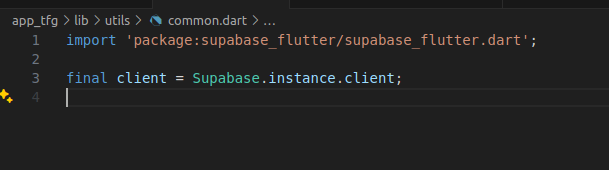
\includegraphics[width=0.7\textwidth]{imagenes/clientBD.png}
	\caption{Instancia de la base de datos.}
	\label{fig:instanciaBD}
\end{figure}

\newpage

\subsection{Tablas de la base de datos}

Las tablas que están dentro de la base de datos son: 


\begin{itemize}
	\item \textbf{clientes:} En esta tabla se almacena toda la información relativa a los clientes. Podemos encontrar campos como el nombre, el teléfono, un comentario para añadir más información y una cartera, que permitirá que el cliente pueda tener dinero negativo o positivo en la tienda. 
	\item \textbf{categorias:} En esta tabla se crean categorías para organizar los artículos dentro de la tienda. Sus atributos tieneTamanio, tieneDescripcion, tieneMaterial, tieneGenero, son booleanos que permiten personalizar los atributos que tendrá un artículo. Si no se seleccionan alguno de estos atributos, todos los artículos que se creen bajo esa categoría no tendrán ese atributo. El atributo nombre indica el nombre de la categoría. 
	\item \textbf{articulos:} En esta tabla se almacena la información de cada uno de los artículos de la tienda. Sus atributos fijos son el nombre, el precio y la subcategoría (que permite categorizar más fino dentro de una categoría y posteriormente filtrar por dichas subcategorías). El resto de atributos son opcionales y se elegirán en la creación de la categoría de dicho artículo. Un artículo representa un modelo, dentro de una prenda podrán haber varias tallas o varios colores, lo que se contempla en la siguiente tabla. 
	\item \textbf{tallas:}  En esta tabla se registran las tallas y los colores disponibles de cada uno de los artículos. Para cada talla se especifica un color, la cantidad actual y la cantidad mínima. La cantidad mínima sirve para detectar cuando un artículo necesita ser renovado. Cuando se tienen igual o menos artículos de los especificados en la cantidad mínima, se mete en una lista de renovación de stock para indicar que deben ser renovados. 
	\item \textbf{movimientos:} En esta tabla se registra toda la información relacionada con los movimientos de la tienda. Se registra el precio total del movimiento, el cliente asignado, el método de pago, la fecha, el tipo de movimiento y el movimiento anterior, este atributo sirve para relacionar unos tickets con otros. Cuando se hace una devolución, se le asigna el movimiento anterior del que procede para poder ver cuál es su procedencia. Además, a las ventas / préstamos también se le asignan las devoluciones para una mejor sincronización.  
	\item \textbf{articulosMov:} En esta tabla se registran todos los artículos que pertenecen a cada movimiento. Es la tabla resultante de una relación muchos a muchos. Además, también se almacena como información adicional, la cantidad comprada de esa talla y el precio parcial. 
\end{itemize}


\subsection{Modificaciones intermedias de la base de datos}

Debido al cambio que solicitó el cliente con las tallas, se tuvo que crear una nueva tabla, la tabla tallas. Esto permitió que un artículo pudiera tener distintas tallas o distintos colores. 


\subsection{Diagrama final del diseño de la base de datos}

En este diagrama podemos ver los atributos que posee cada una de las tablas y como se relacionan entre ellas. Las líneas discontinuas indican las claves externas y los atributos con la llave a la izquierda representan las claves primarias de cada tabla. 

\begin{figure}[H]
	\centering
	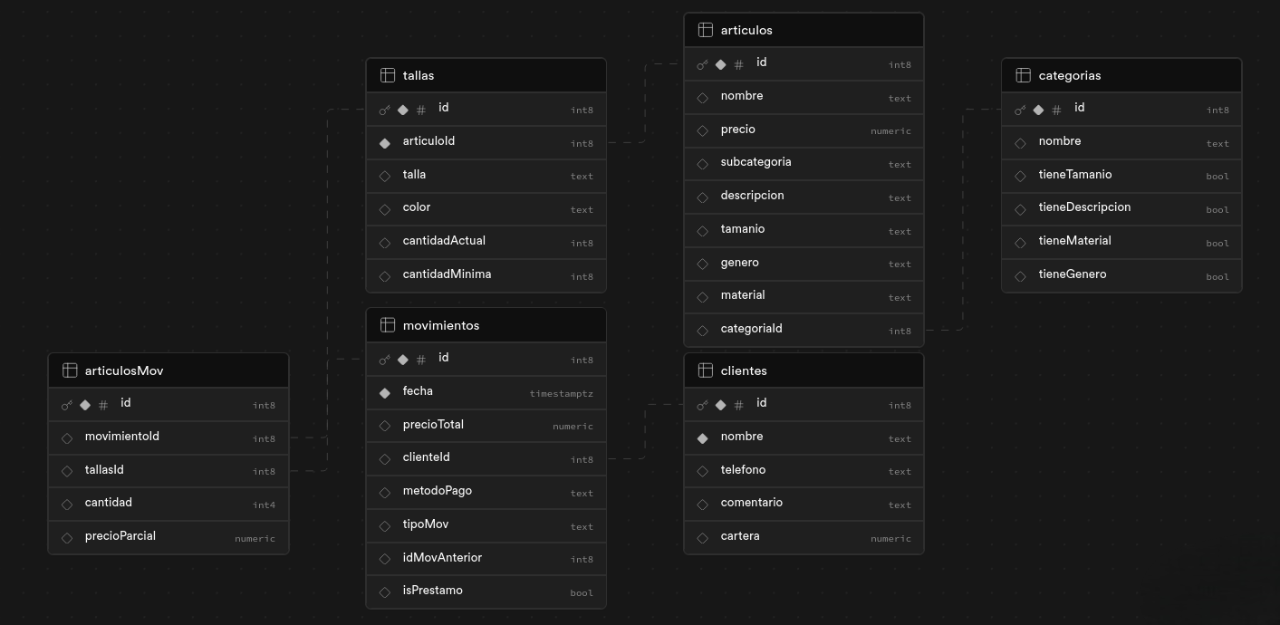
\includegraphics[width=0.7\textwidth]{imagenes/imagenesDiagramas/diagramaBD.png}
	\caption{Diagrama de la base de datos.}
	\label{fig:diagramaBD}
\end{figure}

\section{Diagrama de clases}

Tras finalizar la implementación de la aplicación, se ha construido un diagrama de clases para poder observar las clases que componen el proyecto y las relaciones entre estas. También se pueden ver los atributos y los métodos que tiene cada una de las clases. 

\newpage

\begin{figure}[H]
	\centering
	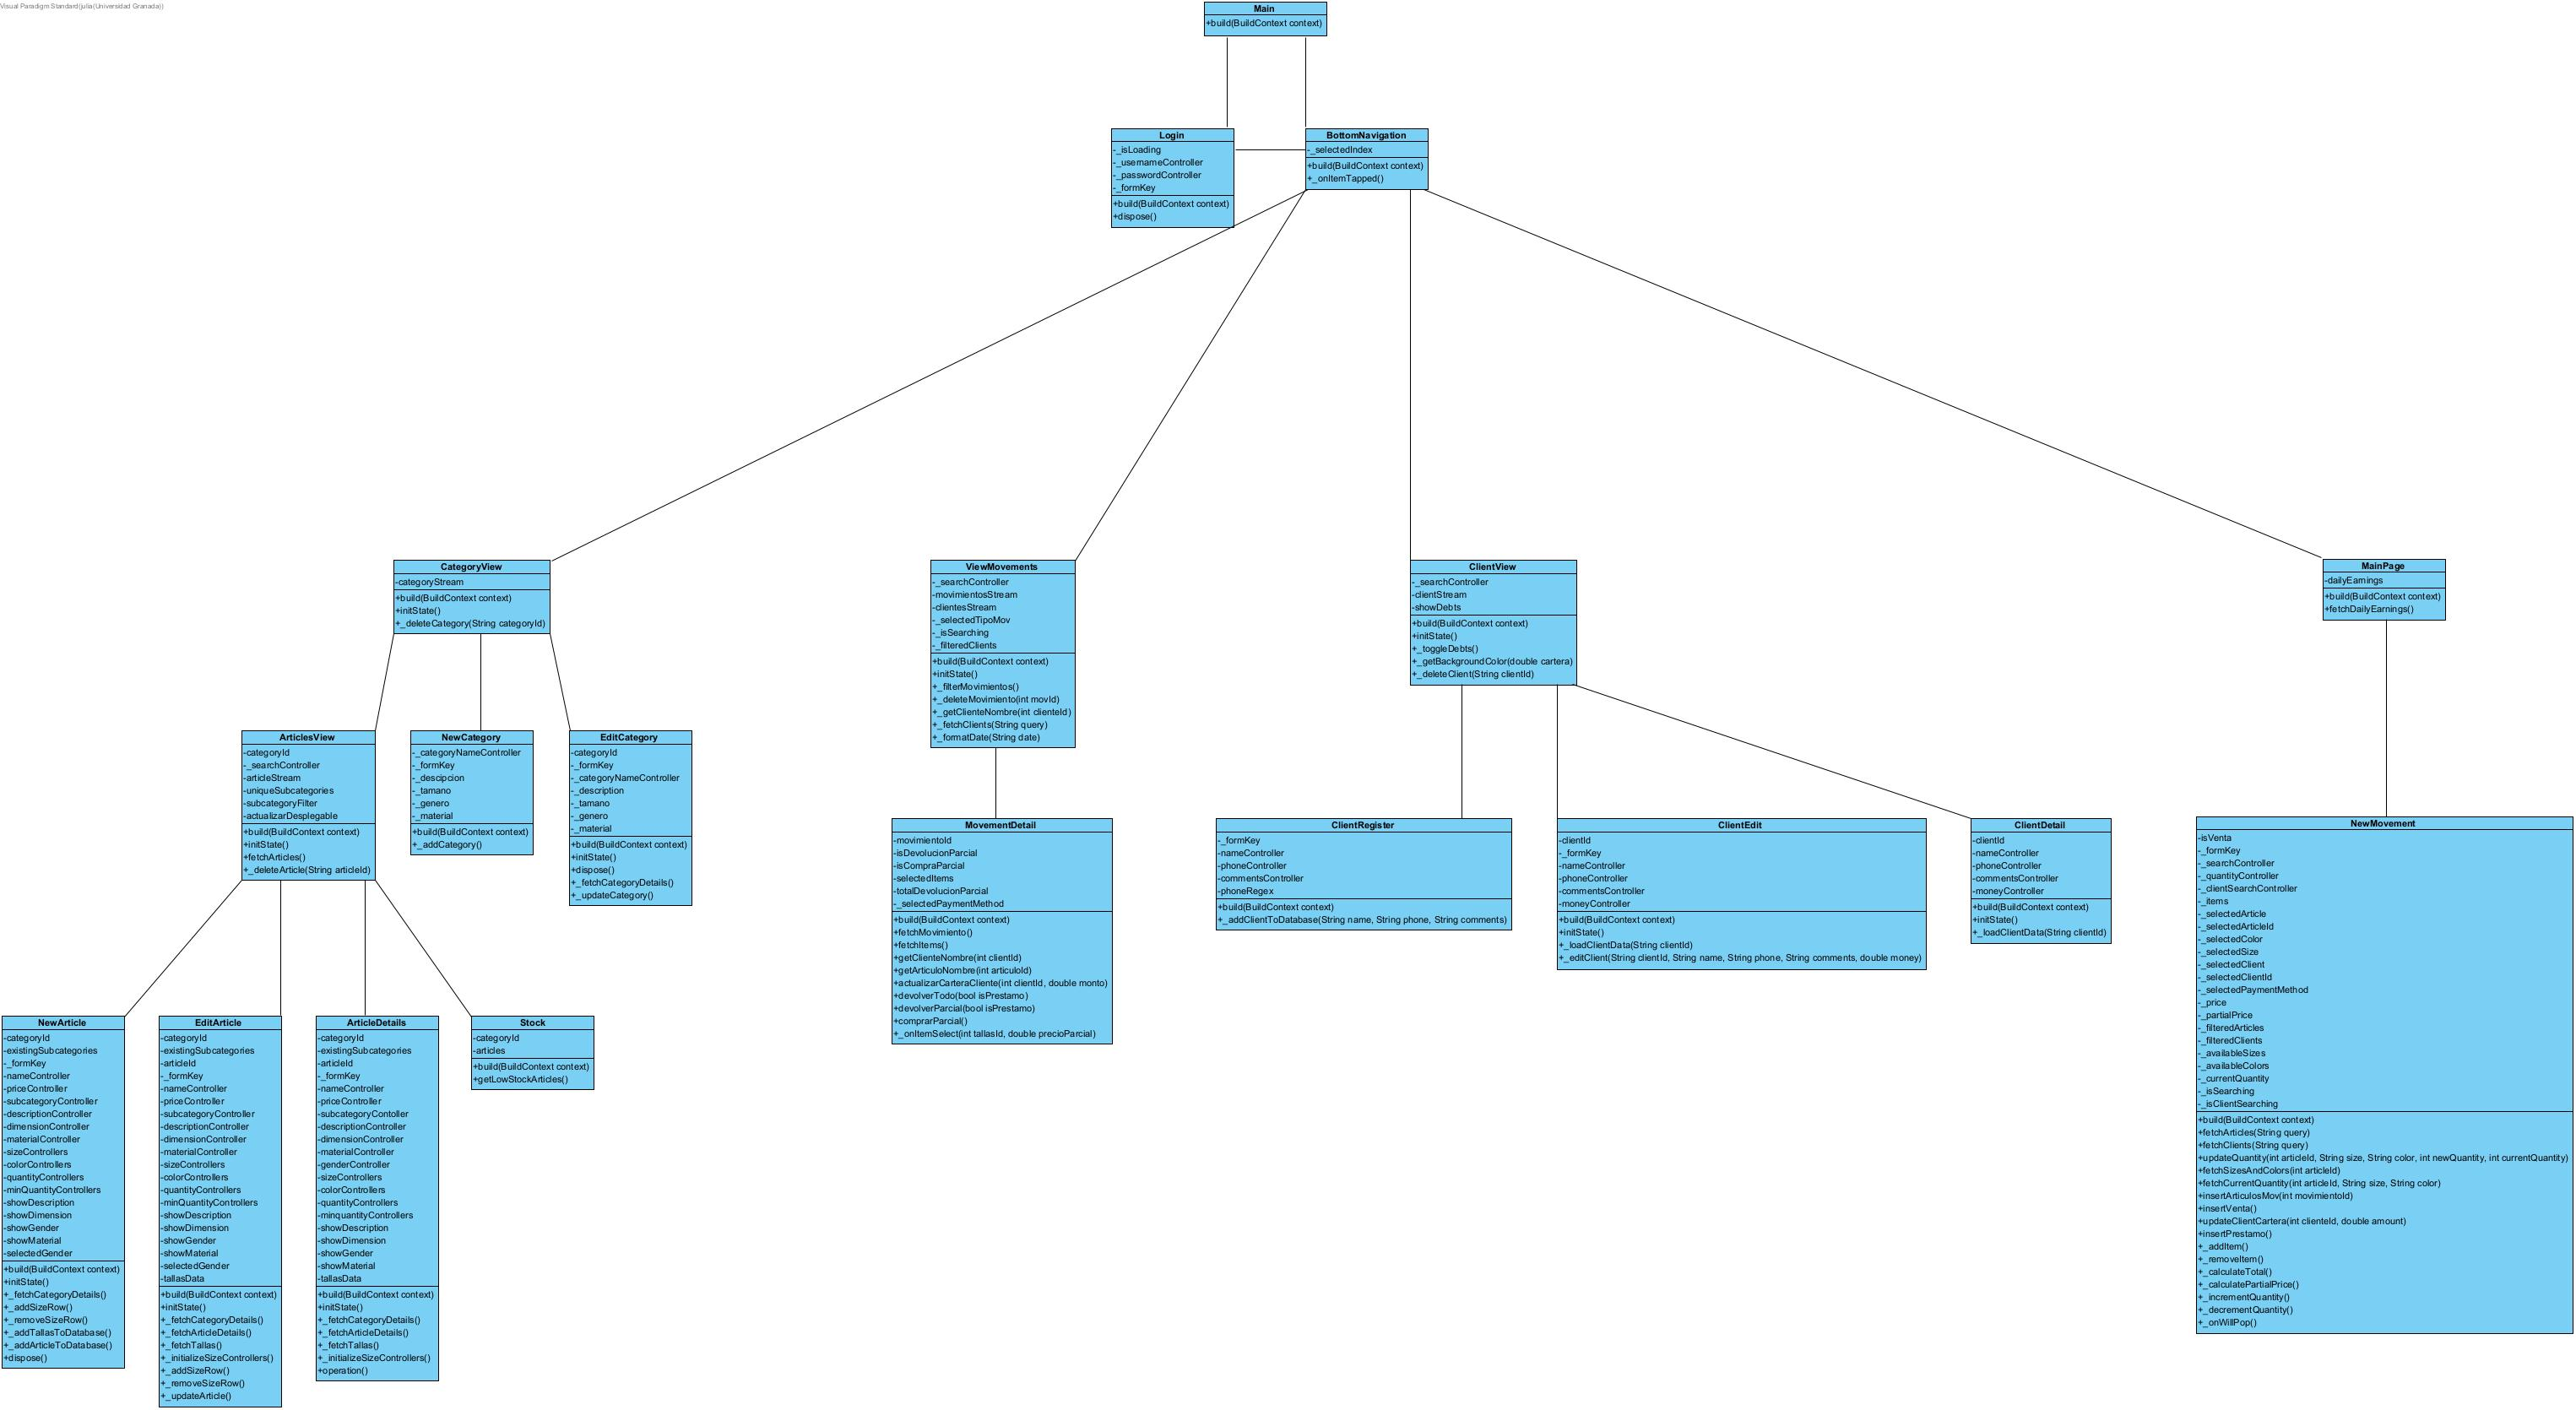
\includegraphics[width=1.1\textwidth, angle=180]{imagenes/imagenesDiagramas/diagramaClases.jpg}
	\caption{Diagrama de clases.}
	\label{fig:diagramaClases}
\end{figure}

\subsubsection{Common}

No es una clase, es un documento donde se declara la instancia de la base de datos. Este documento se importa en cada una de las clases que necesitan la base de datos. De esta forma, hay una única instancia de la base de datos en vez de múltiples instancias. 

\subsubsection{ChangeNotifier}

Es una clase que extiende \textit{ChangeNotifier}, esto permite notificar cambios dentro de la aplicación para poder actualizar las pantallas en los momentos precisos. 

\subsubsection{Main}

En esta clase se define el tema de la aplicación, los colores que se utilizarán en cada widget por defecto. Además, mediante el método \textit{getAuth()} se comprueba si el usuario se ha autenticado. Si no está autenticado, lo redirige a la pantalla de \textit{Login}, mientras que si lo está, lo redirige a la \textit{BottomNav}. 

\subsubsection{Login}

Esta clase, recopila la información mediante los campos de texto de la interfaz gráfica. Cuando tiene el email y la contraseña, los pasa como parámetro al método \textit{signInWithPassword(email, password)} que proporciona la base de datos. Si las credenciales son correctas, el \textit{Main} redirigirá al usuario a la \textit{BottomNav}, mientras que si son incorrectas, mostrará un diálogo informando del error.


\subsubsection{BottomNav}

Esta es la clase de la barra de navegación. Por defecto, cada vez que se inicie sesión, la barra de navegación redirigirá al usuario a la pantalla principal. La barra de navegación tiene 6 iconos con 5 pantallas distintas: la \textit{MainPage}, la \textit{ClientView}, la \textit{CategoryView}, la \textit{MovimientosView} y la \textit{ChartScreen}. El sexto icono se corresponde con el cerrado de sesión. Al pulsar esa opción, aparece un diálogo que pregunta si se quiere cerrar la sesión. Al confirmar el diálogo, se utiliza el método \textit{signOut()} que proporciona la base de datos para cerrar la sesión. 

\subsubsection{Mainpage}

Esta pantalla muestra las ganancias diarias y dos botones que redirigen a la pantalla de \textit{newMovement}, uno para \textit{Nueva venta} y otro para \textit{Nuevo préstamo}. La clase newMovement necesita un booleano para saber si es venta o préstamo, \textit{isVenta}, que se le proporciona en base al botón que se seleccione. 

Para calcular las ganancias diarias, se utiliza el método \textit{fetchDailyEarnings()}. Este método recorre todos los movimientos que se han hecho en el día actual. Suma en una variable los precios totales de las ventas y resta los precios totales de las devoluciones. No se tienen en cuenta los precios totales de los préstamos porque no es dinero que haya entrado en la tienda. Finalmente, asina esa variable a la variable que se muestra por pantalla, \textit{dailyEarnings}. 

\subsubsection{NewMovement}

En esta pantalla, se necesitan varios métodos para cumplir las especificaciones anteriormente comentadas: 

\begin{itemize}
	\item \textbf{fetchArticles(String query)}: Busca artículos dentro de la tabla cuyo nombre contenga la cadena de caracteres proporcionada por parámetro, \textit{query}. 
	\item \textbf{fetchClients(String query)}:  Busca clientes dentro de la tabla cuyo nombre contenga la cadena de caracteres proporcionada por parámetro, \textit{query}. 
	\item \textbf{updateQuantity(int articleId, String size, String color, int newQuantity, int currentQuantity)}: Actualiza la cantidad actual de una artículo para una talla y color específico. 
	\item \textbf{fetchSizesAndColors(int articleId)}: Devuelve las tallas y los colores disponibles para un determinado artículo. 
	\item \textbf{fetchCurrentQuantity(int articleId, String size, String color)}: Devuelve la cantidad actual de un artículo para una talla y un color específico. 
	\item \textbf{insertArticulosMov(int movimientoId)}: Se hace un \textit{insert} para cada artículo de un movimiento. 
	\item \textbf{insertVenta()}: Añade a la tabla \textit{Movimientos} una venta con los datos recolectados de los campos de la interfaz gráfica. 
	\item \textbf{updateClientCartera(int clientId, double amount)}: Actualiza la cartera de un cliente, restándole la cantidad especificada. Esta función se utiliza cuando se crea un nuevo préstamo. 
	\item \textbf{insertPrestamo()}:  Se añade a la tabla \textit(Movimientos) un préstamo con los datos recolectados de los campos de la interfaz gráfica.
	\item \textbf{addItem()}: Comprueba que se hayan completado todos los campos del artículo de forma correcta y lo añade a la lista de artículos del movimiento que se añadirán al finalizar la venta o préstamo. 
	\item \textbf{removeItem()}: Elimina un artículo de la lista de compra. 
	\item \textbf{calculateTotal()}: Calcula el precio total del ticket de compra. 
	\item \textbf{calculatePartialPrice()}: Calcula el precio parcial de cada uno de los artículos de la lista. 
	\item \textbf{incrementQuantity()}: Incrementa la cantidad seleccionada del artículo especificado en una unidad. 
	\item \textbf{decrementQuantity()}: Decrementa la cantidad seleccionada del artículo especificado en una unidad. 
	\item \textbf{onWillPop()}: Este método se llama cuando se desea interrumpir el proceso de creación de un nuevo movimiento. Antes de salir, deshace todos los cambios que se hayan hecho hasta el momento.   
\end{itemize}

\subsubsection{ClientView}

Los métodos necesarios para cumplir con las especificaciones de esta pantalla son:

\begin{itemize}
	\item \textbf{initState()}: Método que se llama al cargar por primera vez la pantalla, hace una llamada a \textit{loadStreams()}.
	\item \textbf{loadStream()}: Hace una consulta a la base de datos para rellenar el \textit{Stream} de clientes. 
	\item \textbf{toggleDebts()}: Cambia de estado la variable de filtrado de clientes que tienen deudas en la tienda. 
	\item \textbf{deleteClient()}: Elimina un cliente si no tiene movimientos vinculados. 
\end{itemize}

\subsubsection{ClientRegister}

El método necesario para cumplir con las especificaciones de esta pantalla es:

\begin{itemize}
	\item \textbf{addClientToDatabase(String name, String phone, String comments)}: Añade el cliente a la base de datos con los valores recogidos a través de los campos de la interfaz gráfica. 
\end{itemize}

\subsubsection{ClientEdit}

Los métodos necesarios para cumplir con las especificaciones de esta pantalla son:

\begin{itemize}
	\item \textbf{initState()}: Método que se llama al cargar por primera vez la pantalla, hace una llamada a \textit{loadClientData(String clientId)}.
	\item \textbf{loadClientData(String clientId)}: Obtiene los datos del cliente seleccionado y asigna esos valores a los campos de texto de la interfaz gráfica. 
	\item \textbf{editClient(String clientId, String name, String phone, String comments, double money)}: Edita los datos del cliente con la información aportada. 
\end{itemize}

\subsubsection{ClientDetail}

Los métodos necesarios para cumplir con las especificaciones de esta pantalla son:

\begin{itemize}
	\item \textbf{initState()}: Método que se llama al cargar por primera vez la pantalla, hace una llamada a \textit{loadClientData(String clientId)}.
	\item \textbf{loadClientData(String clientId)}: Obtiene los datos del cliente seleccionado y asigna esos valores a los campos de texto de la interfaz gráfica. 
\end{itemize}

\subsubsection{CategoryView}

Los métodos necesarios para cumplir con las especificaciones de esta pantalla son:

\begin{itemize}
	\item \textbf{initState()}: Método que se llama al cargar por primera vez la pantalla. Inicializa el \textit{Stream} de categorías mediante una llamada a la base de datos. 
	\item \textbf{deleteCategory(String categoryId)}: Elimina la categoría seleccionada si no tiene ningún artículo vinculado. 
\end{itemize}

\subsubsection{NewCategory}

El método necesario para cumplir con las especificaciones de esta pantalla es:

\begin{itemize}
	\item \textbf{addCategory()}: Añade la categoría a la base de datos con los valores recogidos a través de los campos de la interfaz gráfica. 
\end{itemize}

\subsubsection{EditCategory}

Los métodos necesarios para cumplir con las especificaciones de esta pantalla son:

\begin{itemize}
	\item \textbf{initState()}: Método que se llama al cargar por primera vez la pantalla. Llama al método \textit{fetchCategoryDetails()}. 
	\item \textbf{dispose()}: Hace el \textit{dispose} del controlador del nombre de la categoría. 
	\item \textbf{fetchCategoryDetails()}: Obtiene los datos de la categoría seleccionada y asigna esos valores a los campos de la interfaz gráfica. 
	\item \textbf{updateCategory()}: Edita los datos de la categoría con la información aportada. 
\end{itemize}

\subsubsection{ArticleView}

Los métodos necesarios para cumplir con las especificaciones de esta pantalla son:

\begin{itemize}
	\item \textbf{initState()}: Método que se llama al cargar por primera vez la pantalla. Llama al método \textit{fetchArticles()}. 
	\item \textbf{fetchArticles()}: Obtiene todos los artículos de la categoría seleccionada mediante una consulta a la base de datos. Además, actualiza el \textit{Stream} de artículos con esta información. 
	\item \textbf{deleteArticle(String articleId)}: Elimina el artículo seleccionado si no está vinculado a ningún movimiento. 
\end{itemize}

\subsubsection{NewArticle}

Los métodos necesarios para cumplir con las especificaciones de esta pantalla son:

\begin{itemize}
	\item \textbf{initState()}: Método que se llama al cargar por primera vez la pantalla. Llama a los métodos \textit{fetchCategoryDetails()} y \textit{addSizeRow()}. El último método obliga a que haya mínimo una talla por artículo.  
	\item \textbf{fetchCategoryDetails()}: Obtiene los datos de la categoría y adapta el formulario de nuevo artículo con las flags activas de dicha categoría. 
	\item \textbf{addSizeRow()}: Añade nuevos controladores de texto cuando se invoca. 
	\item \textbf{removeSizeRow(int index)}: Elimina los controladores de texto del índice especificado. 
	\item \textbf{addTallasToDatabase()}: Añade las tallas que se han completado en el formulario a la base de datos. Hace un \textit{insert} por cada talla, con sus detalles correspondientes. 
	\item \textbf{addArticleToDatabase()}: Añade le artículo con los datos recogidos de los campos de la interfaz gráfica a la base de datos. 
	\item \textbf{dispose()}: Hace el \textit{dispose} de todos los controladores utilizados. 
\end{itemize}

\subsubsection{EditArticle}

Los métodos necesarios para cumplir con las especificaciones de esta pantalla son:

\begin{itemize}
	\item \textbf{initState()}:  Método que se llama al cargar por primera vez la pantalla. Llama a los métodos \textit{fetchCategoryDetails()} y \textit{fetchArticleDetails()}. 
	\item \textbf{fetchCategoryDetails()}: Obtiene los datos de la categoría y adapta los campos que se muestran según los flags activos. 
	\item \textbf{fetchArticleDetails()}: Obtiene los datos del artículo e inicializa los campos de la interfaz gráfica con dichos valores. 
	\item \textbf{fetchTallas()}: Obtiene los datos de todas las tallas vinculadas a ese artículo y lo almacena en una variable. 
	\item \textbf{initializeSizeControlers()}: Inicializa todos los controladores de texto de las tallas con la información previamente obtenida. 
	\item \textbf{addSizeRow()}: Añade nuevos controladores de texto cuando se invoca. 
	\item \textbf{removeSizeRow(int index)}: Elimina los controladores de texto del índice especificado. 
	\item \textbf{updateArticle()}: Actualiza los datos del artículo con la información modificada a través de la interfaz gráfica. 
\end{itemize}

\subsubsection{ArticleDetails}

Los métodos necesarios para cumplir con las especificaciones de esta pantalla son:

\begin{itemize}
	\item \textbf{initState()}:  Método que se llama al cargar por primera vez la pantalla. Llama a los métodos \textit{fetchCategoryDetails()} y \textit{fetchArticleDetails()}. 
	\item \textbf{fetchCategoryDetails()}: Obtiene los datos de la categoría y adapta los campos que se muestran según los flags activos. 
	\item \textbf{fetchArticleDetails()}: Obtiene los datos del artículo e inicializa los campos de la interfaz gráfica con dichos valores. 
	\item \textbf{fetchTallas()}: Obtiene los datos de todas las tallas vinculadas a ese artículo y lo almacena en una variable.
	\item \textbf{initializeSizeControlers()}: Inicializa todos los controladores de texto de las tallas con la información previamente obtenida. 
\end{itemize}

\subsubsection{Stock}

El método necesario para cumplir con las especificaciones de esta pantalla es:

\begin{itemize}
	\item \textbf{getLowStockArticles()}: Obtiene una lista de las tallas de los artículos cuya cantidad actual sea igual o inferior a la cantidad mínima establecida. 
\end{itemize}

\subsubsection{MovimientosView}

Los métodos necesarios para cumplir con las especificaciones de esta pantalla son: 

\begin{itemize}
	\item \textbf{initState()}: Método que se llama al cargar por primera vez la pantalla, hace una llamada a \textit{loadStreams()}.
	\item \textbf{loadStreams()}: Hace una consulta a la base de datos para rellenar el \textit{Stream} de movimiento ordenados por fecha y el \textit{Stream} de los clientes ordenados por nombre.  
	\item \textbf{filterMovimientos()}: Vuelve a cargar la página, para que se actualice con los movimientos filtrados. 
	\item \textbf{actualizarCarteraCliente(int clienteId, double monto)}: Actualiza la cartera del cliente, añadiendo el monto a la cantidad actual. Se llama cuando se elimina un movimiento de tipo préstamo.  
	\item \textbf{deleteMovimiento(int movId)}: Se elimina el movimiento especificado si no está vinculado a ningún otro. Además, se actualiza el stock de los artículos que estuvieran dentro del movimiento, se borran las entradas en la tabla \textit{ArticulosMov} que estuvieran relacionados con ese movId y, finalmente, se elimina el movimiento. 
	\item \textbf{getClienteNombre(int clienteId)}: Obtiene el nombre del cliente con ese ID. 
	\item \textbf{fetchClients(String query)}: Obtiene los clientes cuyo nombre contengan la cadena de caracteres pasada por parámetro, \textit{query}. 
	\item \textbf{formatDate()}: Le da formato a la fecha actual. 	
\end{itemize}

\subsubsection{MovementDetail}

Los métodos necesarios para cumplir con las especificaciones de esta pantalla son:
 
\begin{itemize}
	\item \textbf{fetchMovimiento()}: Obtiene la información del movimiento que se va a mostrar en la pantalla mediante una consulta a la base de datos. 
	\item \textbf{fetchItems()}: Obtiene todos los artículos vinculados a ese movimiento. 
	\item \textbf{getClienteNombre(int clienteId)}: Obtiene el nombre de un cliente a partir de su ID. 
	\item \textbf{getArticuloNombre(int articuloId)}: Obtiene el nombre de un artículo a partir de su ID. 
	\item \textbf{actualizarCarteraCliente(int clienteId, double monto)}: Actualiza la cartera del cliente, añadiendo el monto a la cantidad actual. Se llama cuando se devuelve un movimiento de tipo préstamo.  
	\item \textbf{devolverTodo()}: Devuelve todos los artículos de una venta o un préstamo y actualiza el inventario. Si es un préstamo, actualiza la cartera del cliente. Si es una venta, el método de pago de la devolución será igual que el método de pago de la venta. Además, relaciona el movimiento original con el movimiento de devolución para una navegación rápida. 
	\item \textbf{devolverParcial()}: Similar al método \textit{devolverTodo()} pero permite seleccionar los artículos que se desean devolver. Permite seleccionar el método de pago de la devolución. 
	\item \textbf{comprarParcial()}: Este método solo aplica para préstamos. Permite convertir un préstamo en venta, comprando los artículos seleccionados. Los artículos que no se seleccionan, formarán un movimiento de devolución y se actualizará la cartera del cliente con ese precio parcial devuelto. El movimiento original se vinculará con la devolución. Si no hay ninguna devolución porque se han comprado todos los artículos, no se vinculará a ningún movimiento. 
	\item \textbf{onItemSelect(int tallasId, double precioParcial)}: Filtra la lista de artículos y solo se queda con aquellos que estén seleccionados. 
\end{itemize}

\subsubsection{ChartScreen}

Los métodos necesarios para cumplir con las especificaciones de esta pantalla son:

\begin{itemize}
	\item \textbf{initState()}: Método que se llama al cargar por primera vez la pantalla, hace una llamada a \textit{fetchEarnings()}.
	\item \textbf{fetchEarnings()}: Dependiendo del valor seleccionado en el desplegable, mensual o anual, hace una llamada a \textit{fetchMonthlyEarnings()} o \textit{fetchAnnualEarnings()}.
	\item \textbf{fetchMonthlyEarnings()}: Determina los días que hay en el mes y, para cada uno de los días de ese mes, hace un recuento del dinero ganado, sumando el precio total de las ventas y restando el precio total de las devoluciones procedentes de ventas. Las devoluciones procedentes de préstamos no se restan porque es dinero que nunca entró en la tienda. Finalmente vuelve a cargar la pantalla para que se apliquen los cálculos.
	\item \textbf{fetchAnnualEarnings()}:  Realiza un cálculo similar a el mensual, pero en vez de mostrar las ganancias día a día, las muestra mes a mes. Finalmente vuelve a cargar la pantalla para que se apliquen los cálculos.
	\item \textbf{onOptionChanged(String newValue)}: Cambia el valor de la variable que controla el desplegable de la interfaz gráfica. 
\end{itemize}
